\chapter{Pflichtenheft}
Bei der Erstellung dieses Pflichtenheftes wurde sich an folgendem Beispiel von Stefan Baur orientiert. \\
\url{http://www.stefan-baur.de/cs.se.pflichtenheft.beispiel.html?glstyle=2010}

\section{Zielbestimmungen}
\subsection{Projektbeteiligte}
Wer soll an dem Projekt teilnehmen?
\begin{itemize}
        \item Christopher Pahl
        \item Christoph Piechula
        \item Eduard Schneider
        \item Marc Tigges
\end{itemize}
\subsection{Muss-Kriterien}
\renewcommand{\labelitemi}{•}
\begin{itemize}
	\item Verbindungsaufbau
	\item Durchführung benutzerspezifischer Client-Einstellungen
	\item Musik-Steuerung
	\item Warteschlangenverwaltung
	\item Playlistverwaltung
	\item Datenbankverwaltung
	\item Frontend für die Settings
	\item Statistikanzeige
	\item Verwaltung der Ausgabegeräte
\end{itemize}
\subsection{Wunsch-Kriterien}
\begin{itemize}
    \item Anzeige von Onlinecontent (Albencover, Lyrics etc.) unter Verwendung von \href{https://github.com/sahib/glyr}{libglyr}
\end{itemize}

\section{Produkteinsatz}
Der MPD-Client ist nicht auf bestimmte Gewerbe beschränkt, ein jeder soll diesen Client
verwenden können. \\
Die Software soll unter folgender Lizenz stehen:
General Public License Version 3 vom 29 Juni 2007.\ \\ 
Definition der GPL:
\begin{center}
    \url{http://www.gnu.org/licenses/gpl.html}
\end{center}
\subsection{Anwendungsbereiche}
Einzelpersonen verwenden dieses System überall da, wo mit
einem Unixoiden Betriebssystem Musik abgespielt werden soll.
Das wären z.B. Personal Computer, Musikanlagen, Laptops und evtl.
sogar diverse Smartphones möglich.

\subsection{Zielgruppen}
Personengruppen, die komfortabel von überall aus auf ihre Musik und Playlist zugreifen
wollen, ohne diese jedes mal aufwändig synchronisieren zu müssen (z.B. Durch Abgleich von Datenträgern). 
Aufgrund der für das System vorgesehenen Betriebsumgebung sind ebenso Kenntnisse im Umgang mit Unix nötig. 
Der Benutzer muss die Systemsprache Englisch beherrschen.


\subsection{Betriebsbedingungen}
Das System soll sich bezüglich der Betriebsbedingungen nicht sonderlich von vergleichbaren Systemen bzw.
Anwendungen unterscheiden und dementsprechend folgende Punkte erfüllen:
\begin{itemize}
        \item Betriebsdauer: Täglich, 24 Stunden
        \item Keinerlei Wartung soll nötig sein
        \item Sicherungen der Konfiguration müssen vom Benutzer vorgenommen werden
\end{itemize}

\section{Produktumgebung}
\subsection{Software}
\begin{itemize}
	\item Unixoides Betriebssystem
	\item MPD-Server 
	\item Avahi Daemon
	\item Benötigte Bibliotheken können statisch einkompiliert werden
\end{itemize}
Ein MPD-Server muss nicht unbedingt lokal installiert, jedoch dann über das Netzwerk (Internet) erreichbar sein.
Ohne MPD-Server soll der Client in einen definierten Zustand hochgefahren werden der das Verbinden ermöglicht.
Ein laufender Avahi Daemon ist optional. Er ist nicht vonnöten, aber durchaus praktisch, wenn man sich nicht ständig den Host (bzw. die IP) 
vom Administrator geben lassen will und stattdessen in der eingebauten Serverliste nachschauen kann.

\subsection{Orgware}
\begin{itemize}
	\item CMake (Buildsystem)
	\item g++ (C++ Compiler)
	\item Valgrind (Memorydebugger)
	\item git (Hosting auf Github) 
	\item Glade (GUI-Designer)
	\item doxygen  (Interne Dokumentationsgenerierung)
	\item Devhelp (Dokumentationsbrowser)
\end{itemize}

\section{Produktfunktionen}
Funktionen des MPD-Clients.\ \\
Beim ersten Start des Systems soll eine einkompilierte Standard-Konfiguration geladen und die Verbindungseinstellungen
zu einem MPD-Server vorgenommen werden. Bei jedem weiteren Start soll die vom Benutzer erstellte Konfiguration geladen werden.
Falls keine Konfiguration gefunden wurde oder diese beschädigt ist,
wird auf eine vom Client bereitgestellte Standardkonfiguration zurückgegriffen. Der Benutzer soll sämtliche
Einstellungen selbstverständlich zu jeder Zeit ändern können.
\newpage
\paragraph{Mockup:}
Um ein Gefühl für die Funktionalität zu bekommen die der Client haben soll, wurde mit Glade ein nichtfunktionales Mockup erstellt, 
um daraus die finalen Features abzuleiten. 

\begin{figure}[h!]
    \fbox{
    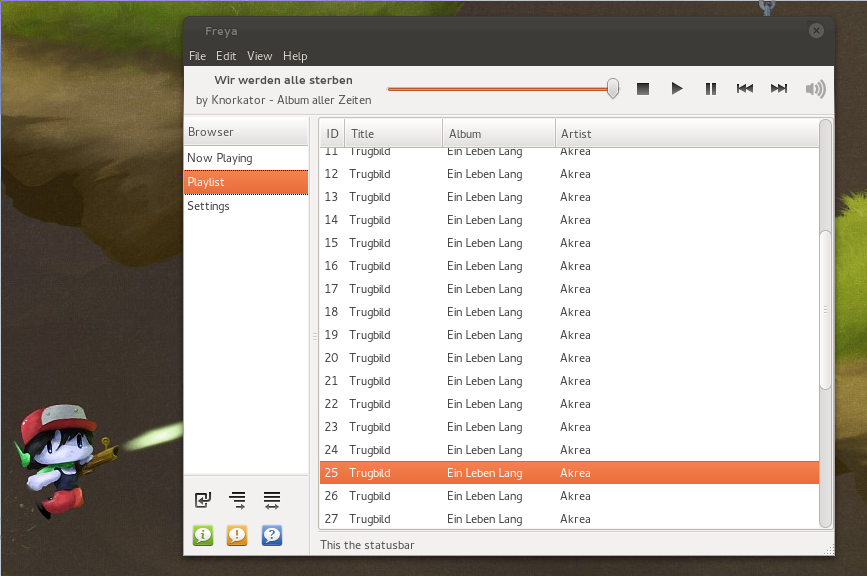
\includegraphics[width=\textwidth]{./gfx/misc/final_mockup.png}}
    \caption{Mockup des MPD Clients}
    \label{p_mockup}
\end{figure}

Die Auflistung der Features erfolgt grob von links oben nach rechts unten. Auf eine Nummerierung der einzelnen Funktionen
wurde verzichtet, da das Designdokument einen leicht anderen Aufbau hat, was das referenzieren erschwert. 

\subsection{Menü}
Überall Anzeige der Keyshortcuts, für jedes relevante Element.
\begin{itemize}
\item File
  \begin{itemize}
  \item ,,Connect''; Ausgegraut wenn bereits verbunden
  \item ,,Disconnect'', Ausgegraut wenn nicht verbunden
  \item ,,Quit''
  \end{itemize} 
\item ,,Playback'' Anzeige mit Haken falls aktiviert 
  \begin{itemize}
  \item Next Song
  \item Previous Song
  \item Play
  \item Stop
  \item Consume, Single, Random, Repeat 
  \end{itemize}   
\item Help
  \begin{itemize}
  \item About Dialog
  \end{itemize}
\end{itemize}

%-------------------------------------------------------------

\subsection{Titelbar}
\begin{itemize}
	\item Anzeige des Musiktitels
	\begin{itemize}
		\item Benutzerhinweis wenn Client nicht verbunden ist
	\end{itemize}
	\item ,,Timeslider''
	\begin{itemize}
		\item Zeigt die aktuelle Liedposition an.
		\item Sprung an bestimmte Musikposition durch Ziehen möglich.
		\item Bei Stop wird Slider auf 0 gesetzt, bei Pause  bleibt dieser stehen.
	\end{itemize}
	\item Steuerbuttons
	\begin{itemize}
		\item Stopbutton - Stoppt Lied, setzt Timeslide zurück auf 0)
        \item Pausebutton - zeigt ein ,,\emph{Play Icon}'' wenn pausiert und ein ,,\emph{Pause Icon}'' bei Wiedergabe
		\item Previous - vorheriges Lied
		\item Next - nächtes Lied
		\item Volumebutton - Popupslider zum regeln der Lautstärke
	\end{itemize}
	\item Untere Zeile
	\begin{itemize}
        \item Anzeige von ,,by (\emph{Artist}) on (\emph{Album}) ((\emph{Erscheinungsjahr - falls vorhanden}))''
        \item Bei Musikstücken die nicht getaggt worden sind, und somit keine Artist oder Album-Informationen anbieten,
            soll der Name der Datei angezeigt werden. 
        \item Falls nicht connected oder nicht spielend soll ,,\emph{Not Playing angezeigt}''
    \end{itemize}		
\end{itemize} 

%-------------------------------------------------------------

\subsection{Sidebar}
Die Sidebar befindet sich links und zeigt eine Liste verfügbarer Browser
\begin{itemize}
    \item Bei Klick auf einem Browser wird er ausgewählt
    \item der Inhalt wird im Pane daneben angezeigt
    \item Sollte die Browserliste überfüllt sein wird ein Scrollbalken angezeigt
\end{itemize}
Nach einem Separator findet sich ein inaktives widget das den Song anzeigt der als nächstes spielen wird.
Falls kein nächster Song wird eine entsprechende Nachricht angezeigt.
Darunter findet sich 4 eindrückbare Buttons die eindrückbar sind:
\begin{itemize}
    \item Repeat
    \item Consume
    \item Repeat
    \item Single
\end{itemize}
Falls diese Buttons beispielsweise in einem anderen Client aktiviert werden, 
so sollen die Änderungen automatisch durch die Eindrückung angezeigt werden.


%-----------------------------------------------

\subsection{Playlistmanager}
\begin{figure}[htb!]
    \centering
    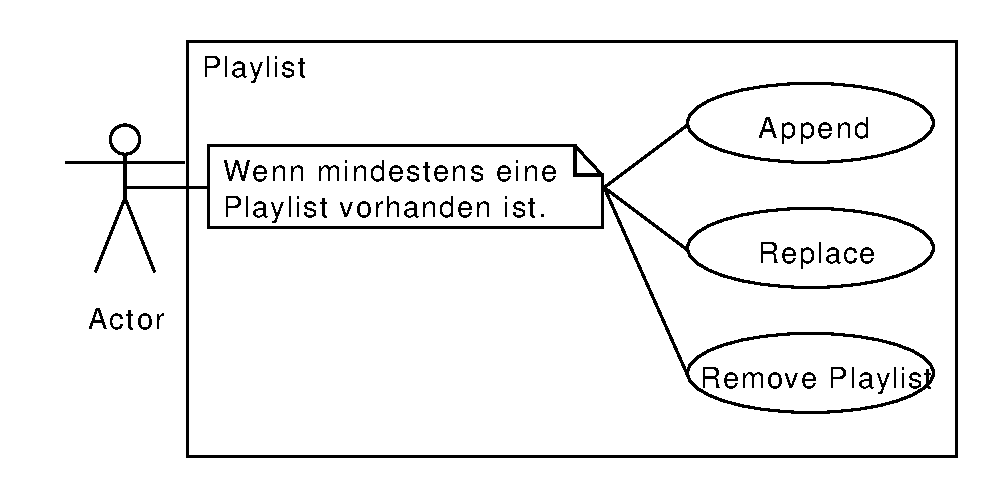
\includegraphics[width=\textwidth]{./gfx/usec/playlist}
    \caption{Use Case Diagramm Playlist}
    \label{uc_playlist}
\end{figure}
Zeigt alle vorhandenen auf dem Server gespeicherten Playlisten in einer Liste.
Dabei wird in der Liste der Playlistname und das letzte Änderungsdatum angezeigt.
Die Namenszellen sind editierbar, sodass der Playlistname einfach geändert werden kann. 
Ein Rechtsklickmenü bietet soll die folgenden Operationen bieten (siehe \ref{uc_playlist}):
\begin{itemize}
    \item \textbf{Append:} Fügt den Inhalt der Playliste der Queue am Ende hinzu
    \item \textbf{Replace:} Ersetzt den Inhalt der Queue mit dieser Playlist
    \item \textbf{Delete:} Entfernt die ausgewählten Playlisten unwiderruflich
\end{itemize}   

%-----------------------------------------------

\subsection{Databasebrowser}
\begin{figure}[htb!]
    \centering
    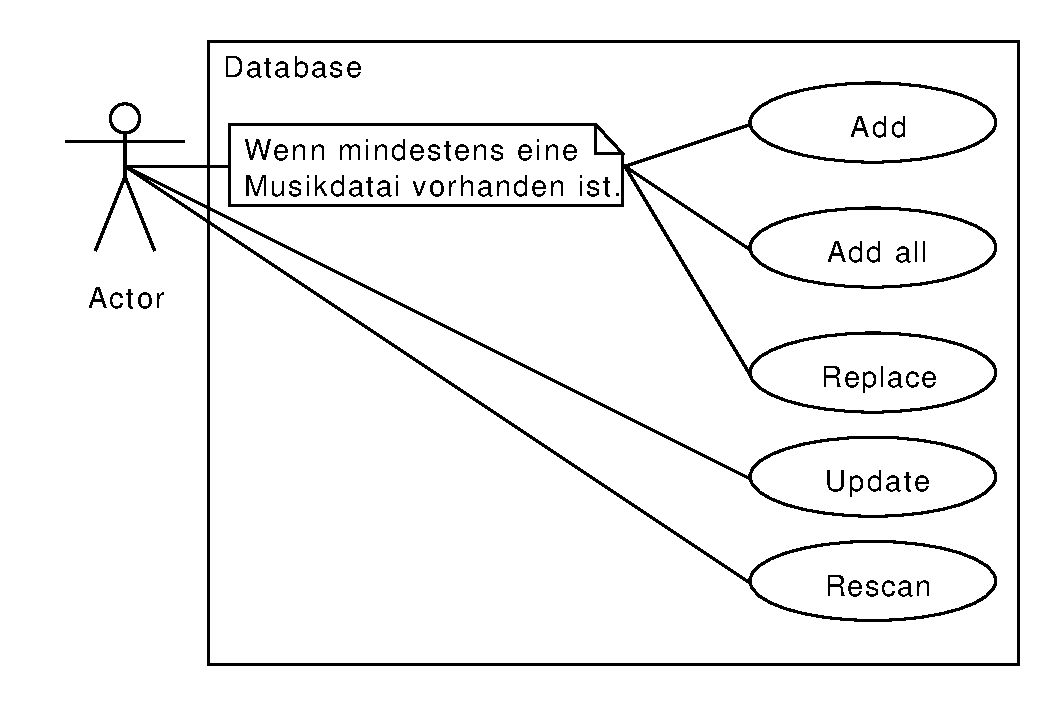
\includegraphics[width=\textwidth]{./gfx/usec/database}
    \caption{Use Case Diagramm Database}
    \label{uc_database}
\end{figure}
Der Databasebrowser zeigt eine Visualisierung der Datenbank die an einen Filebrowser angelehnt ist.
Es handelt sich hierbei nicht wirklich um ein Dateisystem, nur um eine Darstellung der Musikfiles die vom Server angeboten werden.
\begin{itemize}
    \item Anzeige von Songs und Files durch unterschiedliche Icons
    \item Anzeige des "Dateinamen" unter dem Icon
    \item Doppelklick oder Enter auf einen Ordner bewirkt ein Absteigen in diesen
    \item Doppelklick oder Enter auf ein Songfile bewirkt ein Hinzufügen dessen zur Ende der Queue
    \item ''Backspace'' geht ebenso ein Verzeicniss nach oben.
    \item Am unteren Rand befindet sich eine Steuerleiste:
        \begin{itemize}
            \item \textbf{Homebutton:} Geht zum Wurzel-Verzeichnis zurück
            \item \textbf{Zurückbutton:} Dasselbe wie Backspace
            \item Das Suchfeld filtert die momentane Anzeige
            \item ganze rechts zeigt ein Label den aktuellen Pfad an
        \end{itemize}
    \item Ein Kontextmenü bietet folgende Optionen (siehe auch Abb.: \ref{uc_database}):
        \begin{itemize}
            \item \textbf{Add:} Fügt die ausgewählte Menge der Queue hinzu, rekursiv falls sich Verzeichnisse darunter befinden
            \item \textbf{Add All:} Fügt alles, ungeachtet der auswahl der queue hinzu (performamtere Version von add)
            \item \textbf{Replace:} Wie add, löscht aber vorher die Queue
            \item \textbf{Update:} Weist den Server an die Datenbank zu aktualisieren, und neue/veränderte files zu aktualisieren
            \item \textbf{Rescan:} Weist den Server die Datenbank zu aktualisieren; untersucht alle files von neuen (teuere Operation)
        \end{itemize}
\end{itemize}

%-----------------------------------------------

\subsection{Queue}

\begin{figure}[htb!]
    \centering
    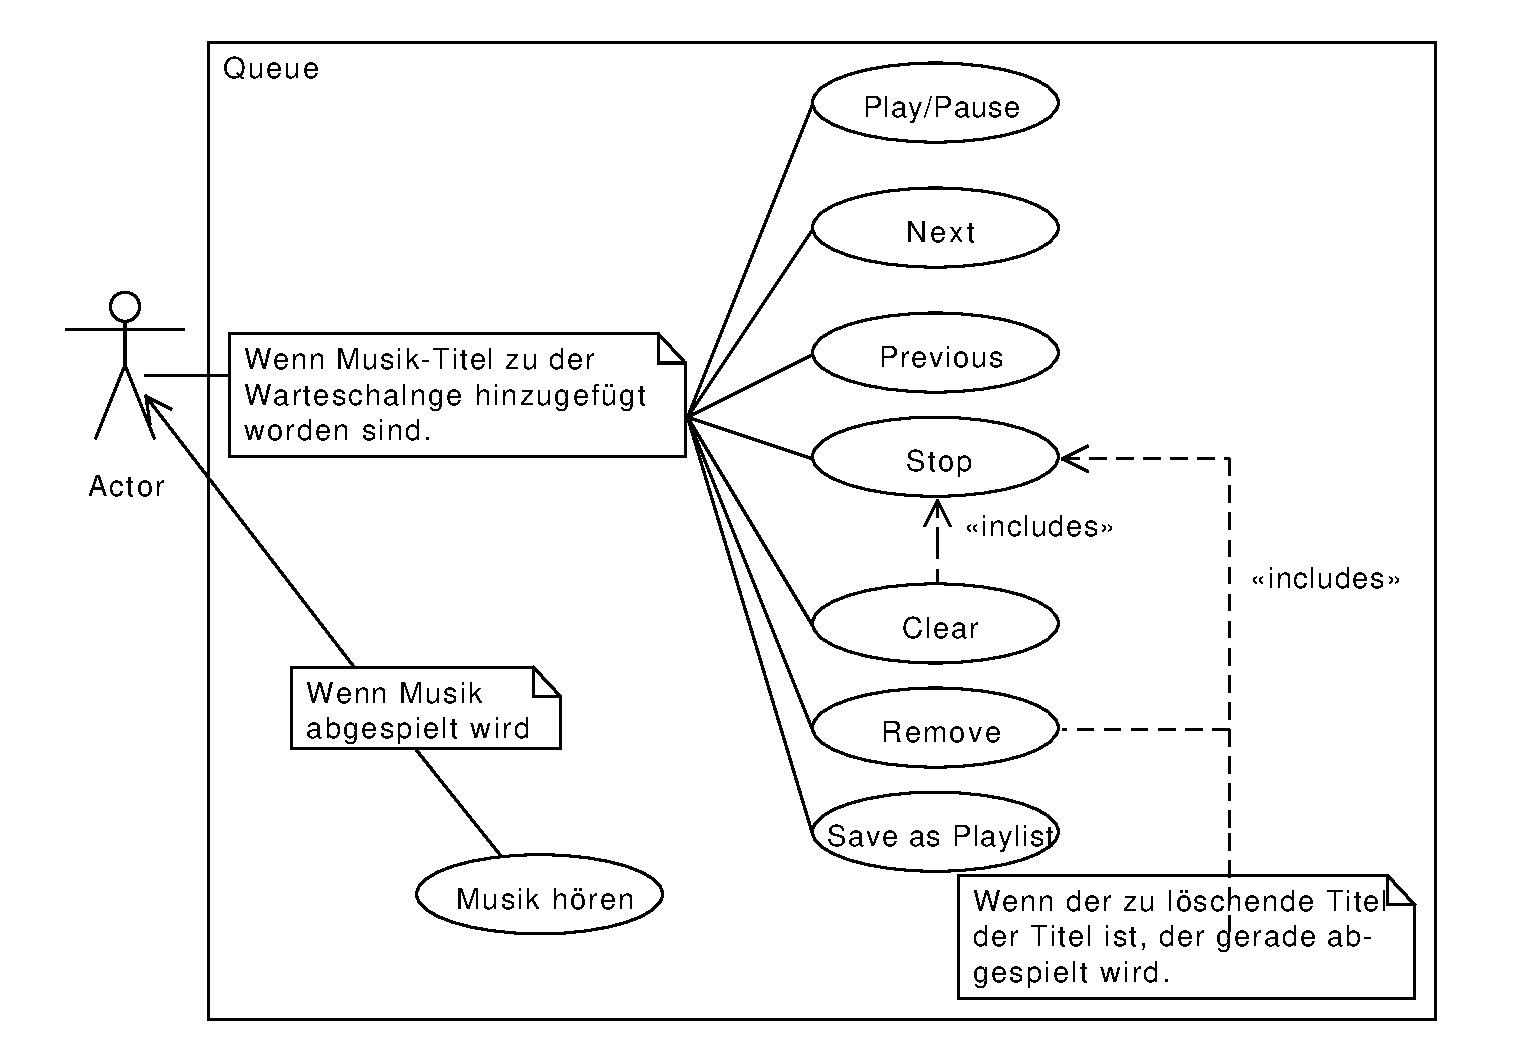
\includegraphics[width=\textwidth]{./gfx/usec/queue}
    \caption{Use Case Diagramm Queue}
    \label{uc_queue}
\end{figure}

\begin{itemize}
    \item Zeigt die aktuelle Warteschlange an
        \begin{itemize}
            \item Künstler, Album und Songtitel 
            \item Spalten der Queue sind frei anordenbar
        \end{itemize}
    \item Auswahl erfolgt durch linksklick (kombiniert mit shift/strg) oder durch Auswählen mit der Maus (,,Rubberbanding'')
    \item Ein Rechtsklickmenü bietet die folgenden Möglichkeiten:
        \begin{itemize}
            \item \textbf{Remove:} Entfernen der Songs aus der Queue
            \item \textbf{Clear:} Entfernen aller Songs aus der Queue
            \item \textbf{Save as playlist:} Die gesamte Queue wird als playlist abgespeichert, \\
                der Name der neuen Playlist wird durch einen Dialog abgefragt.
        \end{itemize}
    \item Bei Änderungen des Server wird die Queue im Hintergrund geupdatet
\end{itemize}

%-----------------------------------------------

\subsection{Settingsbrowser}
Die Einstellungen sollen in ein Tabbasiertes Layout eingebettet sein. 
Werden Änderungen vorgenommen, so werden sie nicht gleich gespeichert und übernommen. 
Es sollte daher ein Speicherfunktion geben, und dazugehörig eine Undofunktion für die letzten Änderungen.
\\
Falls dem Client die Verbindung verloren soll zum Settingsbrowser gesprungen werden, sodass der Benutzer entsprechende
Änderungen machen kann. Aus diesem Grunde muss der Settingsbrowser auch ohne Verbindung voll funktionsfähig sein.
Alle Settingstabs ändern die Werte nicht sofort:
\begin{itemize} 
    \item Sie werden erst persistent übernommen wenn der Benutzer die Konfiguration abspeichert
    \item Der Rückgängigbutton setzt die Präsentation auf die letzen persistent gesetzten Werte
    \item ,,Zurücksetzen'' lädt überall die Defaultconfig
\end{itemize}
Innerhalb der Tabs sollen folgende Funktionen bereit gestellt werden:
\begin{itemize}
    \item Der Benutzer kann Netzwerk-Einstellungen vornehmen
        \begin{itemize}
            \item Server IP / Port
            \item Avahi-Browser
                Anmerkung: Dieser soll eine Liste mit lokalen MPD Servern anzeigen,
                die sich über Zeroconf zu erkennen geben. 
            \item Autoconnect (Verbinde zum letzt eingestellten Server beim Start)
        \end{itemize}
    \item Der Benutzer kann Playback-Einstellungen vornehmen	
        \begin{itemize}
            \item Crossfade in Sekunden (Weicher Übergang zwischen aktuellem und nächstem Lied)
            \item Musik beim verlassen stoppen
        \end{itemize}
    \item Der Benutzer kann Allgemein-Einstellungen vornehmen
        \begin{itemize}
            \item Notifications(libnotify) nutzen, falls ja auch wie lange diese angezeigt werden
            \item Tray-Icon anzeigen
        \end{itemize}
    \item Der Benutzer soll eine Audioausgabeliste haben:
        \begin{itemize}
            \item Innerhalb der Liste soll es Checkboxes geben um den Output entweder an oder auszuschalten
            \item Dies soll nicht verfügbar sein wenn die Verbindung verloren geht
        \end{itemize}
\end{itemize}

\subsubsection{Fußleiste}
Falls verbunden zeigt sie:
\begin{itemize}
    \item Samplingrate in Khz
    \item Audiobitrate in Kbit
    \item Outputart (serverbedingt kann nur Stereo oder Mono angezeigt werden, 5.1 Audiofiles werden auch als Stereo dargestellt)
    \item Zeit aktuell von insgesamt
    \item Anzahl an Songs in der Datenbank
    \item Komplette Abspielzeit der Datenbank
    \item Lautstärke 0-100\%
\end{itemize}
\subsubsection{Sonstiges}
\begin{itemize}
    \item Nächster Song (Seitenleiste)
\end{itemize}

\section{Produktdaten}

\subsection{Starten und Beenden}
\begin{itemize}
    \item Der Benutzer kann das System zu jedem Zeitpunkt starten.
    \item Der Benutzer kann das System zu jedem Zeitpunkt beenden.
    \item Beim ersten Start wird ein Standard-System-Zustand geladen.
    \item Beim Beenden wird der aktuelle System-Zustand gespeichert.
    \item Bei jedem weiteren Start wird der letzte System-Zustand geladen.
\end{itemize}
\subsection{Abspielen von Musik (Buttons)}
Der Benutzer kann
\begin{itemize}
    \item Musik abspielen (Play)
    \item Musik stoppen (Stop)
    \item Musik pausieren (Pause)
    \item Musik vor und zurück schalten (Skip)
    \item Musik vor und zurück spulen (Seek)
    \item Musik zufällig abspielen (Random)
    \item Musik wiederholen (Repeat)
    \item Musik im Consume-Mode abspielen
    \item Musik im Single-Mode abspielen
\end{itemize}
\subsection{Abspielen von Musik (Shortcuts)}
Folgende Shortcut sollen in der finalen Version verfügbar sein:\\
\begin{tabularx}{\textwidth}{|X|X|}
    \hline
    \textbf{Funktion} & \textbf{Shortcut} \\
    \hline
     Play & Ctrl + G \\ 
    \hline
     Stop & Ctrl + S \\ 
    \hline
     Previous & Ctrl + P \\
    \hline
     Next & Ctrl + N \\
    \hline
     Random & Ctrl + Z \\
    \hline
     Single & Ctrl + Y \\ 
    \hline
     Repeat & Ctrl + R \\
    \hline
     Consume & Ctrl + T \\
    \hline 
     Verbinden & Ctrl + C \\
    \hline
     Trennen & Ctrl + D \\
    \hline
     Beenden & Ctrl + Q \\
    \hline
\end{tabularx}


\subsection{Administrator-Funktionen}
Durch das Unix-artige System wird der Administrator-Zugriff geregelt. Sobald sich der Benutzer im Unix System
als Administrator befindet, kann er auch den MPD-Client administrieren. Ein zusätzlicher Administrator-Modus wurde also
nicht implementiert.

\subsection{Suchen in der Queue}
Eine einfache Textsuche zum finden von Titeln, Alben oder Interpreten innerhalb der 
Abspiellisten wurde implementiert. Dabei springt die Markierung des Textes beim 
eingeben von Zeichen in die Suche zu der ersten übereinstimmenden Artist in der 
Queue des Clients. Erst beim bestätigen der Eingabe im Suchfeld wird die Auswahl 
anhand einer Volltextsuche gefiltert. Eine Suche nach ,,Kno'' würde so erst zum Artist ,,Knorkator''
springen, und bei Bestätigung werden alle nicht zutreffenden Songs gefiltert.
\begin{itemize}
    \item Der Benutzer kann seine Queue durchsuchen
    \item Der Benutzer kann sein Dateisystem durchsuchen
\end{itemize}
\subsection{Statistik}
\begin{itemize}
    \item Der Benutzer kann eine gesamt Statistik einsehen
        \begin{itemize}
            \item Anzahl der Interpreten
            \item Anzahl der Alben
            \item Anzahl der Lieder
            \item Musiklänge der Datenbank
            \item Abspielzeit	
            \item Zeit Online bzw. mit MPD verbunden
            \item Letztes Datenbank-Update
        \end{itemize}
\end{itemize}

\subsection{Persönliches Profil}
Da die Software auf Unixoide Systeme beschränkt ist, wurde keine Profil-Verwaltung implementiert. Die
verschiedenen Profile werden durch die verschiedenen User des gesamten Betriebssystems definiert und differenziert.
Für spätere Versionen könnte ergänzend auch ein Serveraddressbuch implementiert werden.
\subsection{Mehrfachstart des Clients}
Gegen mehrfaches Starten ist der Client nicht abgesichert. Die einzige Schnittmengen die mehrere Instanzen des Clients sich teilen 
liegt in der persistenten Datenspeicherung des Logs. Werden die Clients zeitversetzt gestartet sollte hier allerdings kaum etwas passieren. 
\subsection{Persönliche Datenbank}
Eine persönliche Datenbank ist lokal nicht vorhanden. Die Datenbank des Benutzers befindet sich auf dem MPD-Server.
Einzig und alleine modulare Erweiterungen des MPD-Clients können lokale Datenbank-Implementierungen erfordern, um
beispielsweise zusätzliche Informationen wie ein ,,Rating'' zu speichern, oder die Suche zu beschleunigen.
\subsection{Persönliche Einstellungen}
Client Einstellungen werden lokal gespeichert, außerdem ist stets eine Defaultconfig vorhanden, falls die des Dateisystems defekt ist.
Die Konfigurationsdatei wird nach dem XDG-Standard in \emph{~/.config/freya/config.xml} gespeichert. Den selben Speicherplatz wählt auch die Logdatei 
(\emph{~/.config/freya/log.txt}). Sollten nur einzelne Werte in der Konfigurationsdatei nicht vorhanden sein so wird nachgeschaut ob die Defaultconfig
diese Werte bereitstellt und es wird versucht sie von dort zu laden. So ist für valide Wert stets abgesichert dass mindestens ein Wert vorliegt.
\section{Qualitätsanforderungen}
Die Software soll natürlich von hoher Qualität sein. Hierfür sollen folgende
Anforderungen erfüllt werden:
\subsection{Korrektheit}
Die Software muss möglichst fehlerfrei und korrekt sein. Es wurden Testszenarien und Testfälle erstellt,
um Fehler zu finden und auszubessern. Aber auch wenn nach Veröffentlichung der Software ein 
Fehler gefunden werden sollte, wird dieser sofort ausgebessert. Bei schwerwiegenden Fehlern
werden die Nutzer direkt auf den Fehler aufmerksam gemacht.
\subsection{Wartbarkeit}
Der Wartungsaufwand der Software ist gering bis gar nicht vorhanden. Ändert sich die Umgebungssoftware
(z.B. der MPD-Server) dann sind die Änderungen so geringfügig bzw. trivial, dass sie den MPD-Client 
nicht beeinflussen werden. Fehler der Software (sollten Fehler auftreten) wären leicht analysiert bzw.
prüfbar und natürlich auch leicht zu beheben. Zur Wartbarkeit gehört ebenso die Modularität, d.h.
die Software ist technisch so realisiert, dass sie leicht erweitert werden kann - Stichwort ModelViewController (MVC). 
\subsection{Zuverlässigkeit}
Das System funktioniert und reagiert tolerant auf fehlerhafte Eingaben bzw. fehlerhafte Benutzung.
Das Programm funktioniert sieben Tage die Woche und 24 Stunden am Tag und muss nicht abgeschaltet werden.

\subsection{Effizienz}
Der MPD-Client funktioniert möglichst effizient, d.h. Das Programm ist schnell geladen und Eingaben des Benutzers
werden praktisch sofort ausgeführt. Es gibt so gut wie keine Wartezeiten, jedenfalls sind diese 
so genannten Reaktionszeiten für den Benutzer nicht merkbar. Selbst bei sehr großen Musik-Datenbanken
und Playlists benötigt das Programm kaum Rechenzeit und sonstige Hardwareressourcen.

\subsection{Benutzbarkeit}
Die Software ist leicht verständlich und intuitiv bedienbar. Nötige Kenntnisse zur Nutzung des 
MPD-Clients sind leicht zu erlernen. Hier wird allerdings davon ausgegangen dass der MPD Server bereits
fertig eingerichtet ist. Sollte dies nicht der Falls sein, so sind Fähigkeiten in der Kommandozeile 
durchaus hilfreich.

\subsection{Design}
Das Design soll ansprechend und modern sein, allerdings wenn es Konflikte zwischen technischer Umsetzung 
und Design oder Effizienz und Design geben sollte, ist stets im Interesse der technischen Umsetzung bzw. 
der Effizienz zu entscheiden.
\subsection{Hardware}
Minimale Hardwareanforderungen: 500 Mhz, 512MB Ram, Festplattenspeicher < 20MB
Empfohlene Hardwareanforderungen: 1 Ghz, 512MB Ram, Festplattenspeicher < 20MB

\subsection{Orgware und Entwicklungsumgebung}
\begin{itemize}
    \item CMake (Buildsystem)
    \item g++ (C++ Compiler)
    \item Valgrind (Memorydebugger)
    \item git (Hosting auf Github) \footnote{https://github.com/studentkittens/Freya}
    \item Glade (GUI-Designer)
    \item doxygen  (Interne Dokumentationsgenerierung)
    \item Devhelp (Dokumentationsbrowser)
    \item Unixodes Betriebssystem
    \item MPD-Server	
    \item Avahi-Browser
    \item gcc (Compiler)
    \item libmpdclient
    \item gtkmm libraries
\end{itemize}
\newpage
